\question{Влияние пространственного заряда на токопрохождение в плоском диоде.
  Уравнение Ленгмюра. Вакуумный диод}

Вакуумный диод считается плоским, если длина и ширина пластин катода и анода
много больше, чем расстояние между ними.
\begin{figure}[h!]
  \center
%  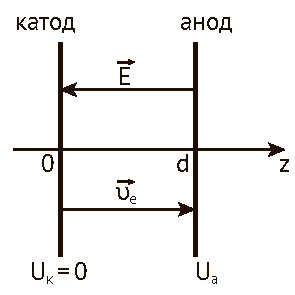
\includegraphics[width=.3\textwidth]{19_diode} \hspace{1em}
%  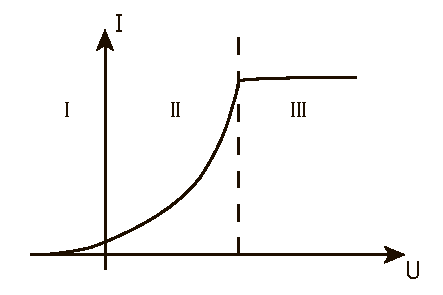
\includegraphics[width=.45\textwidth]{19_VAC} \\
  \parbox{.3\textwidth}{\caption{Схема плоского диода} \label{pic19diode}}
    \hspace{1em}
  \parbox{.45\textwidth}{\caption{Вольт-амперная характеристика диода}
    \label{pic19VAC}} \\
  \parbox{.35\textwidth}{\ } \hspace{1em}
  \parbox{.6\textwidth}{\footnotesize I~-- режим начальных токов~-- ток
    образуется наиболее быстрыми термоэлектронами, способными преодолеть
    тормозящее поле; II~-- режим пространственного заряда~-- ток определяется
    уравнением Ленгмюра~\eqref{eq19Lang}; III~-- область насыщения~-- ток,
    проходящий через диод, равен току термоэлектронной эмиссии}
\end{figure}

Без учета сил пространственного заряда (в т.~н. \emph{холодных} диодных
системах) распределение потенциала описывается выражением (рис.~\pic{19Uz},
штриховая линия):
\[
  U(z) = U_A \cdot \frac{z}{d}.
\]

Рассмотрим плоский диод с учетом сил пространственного заряда (т.~н.
\emph{горячую} диодную систему), предполагая, что начальная скорость всех
электронов равна нулю. Тогда:
\[
  E_z = -\pder{U}{z}; \quad \pder{U}{x} = \pder{U}{y} = 0.
\]

Граничные условия:
\[
  U(z = 0) = 0, \qquad E(z = 0) = -\left. \pder{U}{z} \right|_{z = 0} = 0.
\]

Уравнение Пуассона:
\begin{equation}
  \D U = -\rho / \Ez; \qquad \ppder{}{z}U = -\rho / \Ez.
  \label{eq19puas}
\end{equation}

Найдем плотность пространственного заряда из плотности тока:
\[
  j = -\rho v; \quad \rho = -j / v; \quad v = \sqrt{2 \frac{e}{m} U}; \quad
    \rho = -\sqrt{\frac{m}{2eU}} j.
\]

Подставляя в \eqref{eq19puas}, получим::
\[
  \ppder{}{z} U = \frac{j}{\Ez} \sqrt{\frac{m}{2e}} \frac{1}{\sqrt{U}} =
    \frac{c}{\sqrt{U}}.
\]

Таким образом,
\( \displaystyle
  \ppder{U}{z} = \frac{c}{\sqrt{U}}
\).
Домножим на
\( \displaystyle
  2\pder{U}{z}
\):
\begin{gather*}
  2\pder{U}{z}\ppder{U}{z} = \frac{c}{\sqrt{U}} \cdot 2\pder{U}{z}. \\
  \pder{}{z} \left[ \left( \pder{U}{z} \right)^2 \right] = 4c\cdot
  \pder{}{z} \Big( \sqrt{U} \Big).
\end{gather*}

Интегрируя по \( z \), учитывая второе ГУ:
\[
  \left( \pder{U}{z} \right)^2 = 4c\sqrt{U}; \qquad
  \pder{U}{z} = 2\sqrt{c\sqrt{U}}; \qquad
  \frac{\partial U}{U^{1 / 4}} = 2\sqrt{c}\,\partial z.
\]

Интегрируем, учитывая первое ГУ:
\[
  U^{3 / 4} = \frac{3}{2} \sqrt{c}z.
\]

Подставляя значение константы \( c \), получим:
\begin{equation}
  U^{3 / 4} = \frac{3}{2} \sqrt{\frac{j}{\Ez}\sqrt{\frac{m}{2e}}}z \qquad
  \text{ или (с учетом } I = jS) \qquad
  I = \frac{4}{9} \sqrt{2\frac{e}{m}} \frac{S\Ez}{z^2} U^{3 / 2}.
  \label{eq19UnI}
\end{equation}

В плоскости анода (\( z = d \)) \( U(z = d) = U_A \) уравнение \eqref{eq19UnI}
преобразуется к виду
\begin{equation}
  I_A = \frac{4}{9} \sqrt{2\frac{e}{m}} \frac{S\Ez}{d^2} \cdot U_A^{3 / 2} =
  P \cdot U_A^{3 / 2}.
  \label{eq19Lang}
\end{equation}

Уравнение \eqref{eq19Lang} носит название уравнения <<степени трех вторых>> или
уравнения Ленгмюра и определяет зависимость величины анодного тока \( I_A \) от
значения потенциала на аноде \( U_A \). Величина \( P \) называется первеансом
и зависит от геометрии диода.

\begin{figure}[h!]
  \center
%  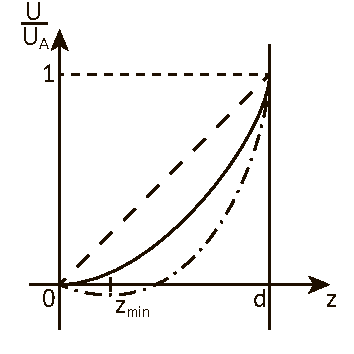
\includegraphics[width=.3\textwidth]{19_Uz} \hspace{.2\textwidth}
%  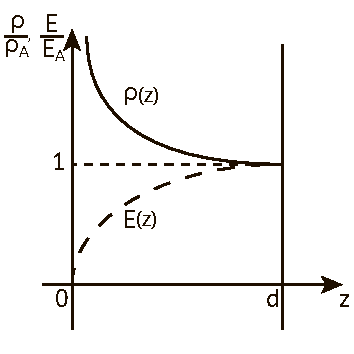
\includegraphics[width=.3\textwidth]{19_Ez} \\
  \parbox{.48\textwidth}{\caption{Распределение потенциала в диодном промежутке}
    \label{pic19Uz}} \hspace{1em}
  \parbox{.48\textwidth}{\caption{Распределение напряженности электрического поля
    и величины пространственного заряда в диодном промежутке} \label{pic19Ez}}
\end{figure}

Из \eqref{eq19UnI} следует, что распределение потенциала вдоль оси \( 0z \)
подчиняется закону
\begin{equation}
  U(z) = U_A \left( \frac{z}{d} \right)^{4 / 3}
  \label{eq19UzUa}
\end{equation}
(рис.~\pic{19Uz}, сплошная линия); распределение пространственного заряда~--
закону
\[
  \rho(z) = \rho_A \left( \frac{d}{z} \right)^{2 / 3}
\]
(рис.~\pic{19Ez}, сплошная линия), где \( \rho_A \)~-- плотность
пространственного заряда на аноде
\(
  \left( \rho_A = \dfrac{4\Ez}{9} \dfrac{U_A}{d^2} \right)
\),
а изменение напряженности электрического поля~-- закону
\[
  E(z) = E_A \left( \frac{z}{d} \right)^{1 / 3}
\]
(рис.~\pic{19Ez}, штриховая линия), где
\(
  E_A = \dfrac{4}{3} \dfrac{U_A}{d}
\).

Идеализация распределения потенциала при наличии пространственного заряда
\eqref{eq19UzUa} связана с тем, что не учитываются начальные скорости электронов
при их вылете с катода. Поэтому, даже при подаче на анод отрицательного
относительно катода напряжения возможно появление анодного тока
(рис.~\pic{19VAC}I). Однако те электроны, которые могут по своим энергетическим
параметрам покинуть катод, но не могут преодолеть тормозящего поля между анодом
и катодом, сосредотачиваются вблизи катода, создавая дополнительное облако
пространственного заряда. Это приводит к понижению потенциала вблизи катода,
появлению <<потенциальной ямы>>, препятствующей электронам, покидающим катод,
достигнуть анода. Это явление называется <<\emph{виртуальным катодом}>>
(рис.~\pic{19Uz}, штрих-пунктирная линия). Его положение \( z_{\min} \) является
положением минимума потенциала. За плоскость виртуального катода вылетают
электроны, начальная скорость которых превышает величину
\(
  v_{\min} \geq \sqrt{2\dfrac{e}{m}U_{\min}}
\),
в связи с чем величина анодного тока должна определяться из соотношения
\[
  I_A = \frac{4}{9} \sqrt{2\frac{e}{m}} \frac{S\Ez}{(d - z_{\min})^2}
  \Big( U_A + \abs{U_{\min}} \Big)^{3 / 2}.
\]
